% Template for PLoS
% Version 3.5 March 2018
%
% % % % % % % % % % % % % % % % % % % % % %
%
% -- IMPORTANT NOTE
%
% This template contains comments intended 
% to minimize problems and delays during our production 
% process. Please follow the template instructions
% whenever possible.
%
% % % % % % % % % % % % % % % % % % % % % % % 
%
% Once your paper is accepted for publication, 
% PLEASE REMOVE ALL TRACKED CHANGES in this file 
% and leave only the final text of your manuscript. 
% PLOS recommends the use of latexdiff to track changes during review, as this will help to maintain a clean tex file.
% Visit https://www.ctan.org/pkg/latexdiff?lang=en for info or contact us at latex@plos.org.
%
%
% There are no restrictions on package use within the LaTeX files except that 
% no packages listed in the template may be deleted.
%
% Please do not include colors or graphics in the text.
%
% The manuscript LaTeX source should be contained within a single file (do not use \input, \externaldocument, or similar commands).
%
% % % % % % % % % % % % % % % % % % % % % % %
%
% -- FIGURES AND TABLES
%
% Please include tables/figure captions directly after the paragraph where they are first cited in the text.
%
% DO NOT INCLUDE GRAPHICS IN YOUR MANUSCRIPT
% - Figures should be uploaded separately from your manuscript file. 
% - Figures generated using LaTeX should be extracted and removed from the PDF before submission. 
% - Figures containing multiple panels/subfigures must be combined into one image file before submission.
% For figure citations, please use "Fig" instead of "Figure".
% See http://journals.plos.org/plosone/s/figures for PLOS figure guidelines.
%
% Tables should be cell-based and may not contain:
% - spacing/line breaks within cells to alter layout or alignment
% - do not nest tabular environments (no tabular environments within tabular environments)
% - no graphics or colored text (cell background color/shading OK)
% See http://journals.plos.org/plosone/s/tables for table guidelines.
%
% For tables that exceed the width of the text column, use the adjustwidth environment as illustrated in the example table in text below.
%
% % % % % % % % % % % % % % % % % % % % % % % %
%
% -- EQUATIONS, MATH SYMBOLS, SUBSCRIPTS, AND SUPERSCRIPTS
%
% IMPORTANT
% Below are a few tips to help format your equations and other special characters according to our specifications. For more tips to help reduce the possibility of formatting errors during conversion, please see our LaTeX guidelines at http://journals.plos.org/plosone/s/latex
%
% For inline equations, please be sure to include all portions of an equation in the math environment.  For example, x$^2$ is incorrect; this should be formatted as $x^2$ (or $\mathrm{x}^2$ if the romanized font is desired).
%
% Do not include text that is not math in the math environment. For example, CO2 should be written as CO\textsubscript{2} instead of CO$_2$.
%
% Please add line breaks to long display equations when possible in order to fit size of the column. 
%
% For inline equations, please do not include punctuation (commas, etc) within the math environment unless this is part of the equation.
%
% When adding superscript or subscripts outside of brackets/braces, please group using {}.  For example, change "[U(D,E,\gamma)]^2" to "{[U(D,E,\gamma)]}^2". 
%
% Do not use \cal for caligraphic font.  Instead, use \mathcal{}
%
% % % % % % % % % % % % % % % % % % % % % % % % 
%
% Please contact latex@plos.org with any questions.
%
% % % % % % % % % % % % % % % % % % % % % % % %

\documentclass[10pt,letterpaper]{article}
\usepackage[top=0.85in,left=2.75in,footskip=0.75in]{geometry}

% amsmath and amssymb packages, useful for mathematical formulas and symbols
\usepackage{amsmath,amssymb}

% Use adjustwidth environment to exceed column width (see example table in text)
\usepackage{changepage}

% Use Unicode characters when possible
\usepackage[utf8x]{inputenc}

% textcomp package and marvosym package for additional characters
\usepackage{textcomp,marvosym}

% cite package, to clean up citations in the main text. Do not remove.
\usepackage{cite}

% Use nameref to cite supporting information files (see Supporting Information section for more info)
\usepackage{nameref,hyperref}

% line numbers
\usepackage[right]{lineno}

% ligatures disabled
\usepackage{microtype}
\DisableLigatures[f]{encoding = *, family = * }

% color can be used to apply background shading to table cells only
\usepackage[table]{xcolor}

% array package and thick rules for tables
\usepackage{array}

% create "+" rule type for thick vertical lines
\newcolumntype{+}{!{\vrule width 2pt}}

% create \thickcline for thick horizontal lines of variable length
\newlength\savedwidth
\newcommand\thickcline[1]{%
  \noalign{\global\savedwidth\arrayrulewidth\global\arrayrulewidth 2pt}%
  \cline{#1}%
  \noalign{\vskip\arrayrulewidth}%
  \noalign{\global\arrayrulewidth\savedwidth}%
}

% \thickhline command for thick horizontal lines that span the table
\newcommand\thickhline{\noalign{\global\savedwidth\arrayrulewidth\global\arrayrulewidth 2pt}%
\hline
\noalign{\global\arrayrulewidth\savedwidth}}



%%  Packages added by Colin
% /* cSpell:enable */
% Symbols
\usepackage{amsmath,amssymb,url,bm}
% Formatting
\usepackage{multicol, csquotes, scrextend, color}   %, titlesec
%% Tables, Figures
\usepackage{longtable, booktabs, pdflscape, placeins, nicematrix, tikz}
\usetikzlibrary{shapes.geometric, arrows}
\tikzstyle{org} = [ellipse, minimum width=3cm, minimum height=0.75cm, text centered, draw=black]
\tikzstyle{io} = [rectangle, minimum width=3cm, minimum height=0.75cm, text centered, draw=black]
\tikzstyle{process} = [rectangle, rounded corners, minimum width=3cm, minimum height=0.75cm, text centered, draw=black]
\tikzstyle{arrow} = [thick,->,>=stealth]

% Images
\usepackage{graphicx, float, caption, subcaption}

% package added by Oster for editing
\usepackage{color} 
\newcommand{\red}[1]{{\color{red}{#1}}}





% Remove comment for double spacing
%\usepackage{setspace} 
%\doublespacing

% Text layout
\raggedright
\setlength{\parindent}{0.5cm}
\textwidth 5.25in 
\textheight 8.75in

% Bold the 'Figure #' in the caption and separate it from the title/caption with a period
% Captions will be left justified
\usepackage[aboveskip=1pt,labelfont=bf,labelsep=period,justification=raggedright,singlelinecheck=off]{caption}
\renewcommand{\figurename}{Fig}

% Use the PLoS provided BiBTeX style
% Colin commented this out - added where bibliography is inserted
% \bibliographystyle{plos2015}

% Remove brackets from numbering in List of References
\makeatletter
\renewcommand{\@biblabel}[1]{\quad#1.}
\makeatother

% Header and Footer with logo
\usepackage{lastpage,fancyhdr,graphicx}
\usepackage{epstopdf}
%\pagestyle{myheadings}
\pagestyle{fancy}
\fancyhf{}
%\setlength{\headheight}{27.023pt}
%\lhead{\includegraphics[width=2.0in]{PLOS-submission.eps}}
\rfoot{\thepage/\pageref{LastPage}}
\renewcommand{\headrulewidth}{0pt}
\renewcommand{\footrule}{\hrule height 2pt \vspace{2mm}}
\fancyheadoffset[L]{2.25in}
\fancyfootoffset[L]{2.25in}
\lfoot{\today}

%% Include all macros below

\newcommand{\lorem}{{\bf LOREM}}
\newcommand{\ipsum}{{\bf IPSUM}}

%% END MACROS SECTION

\begin{document}

\begin{figure}[!h]
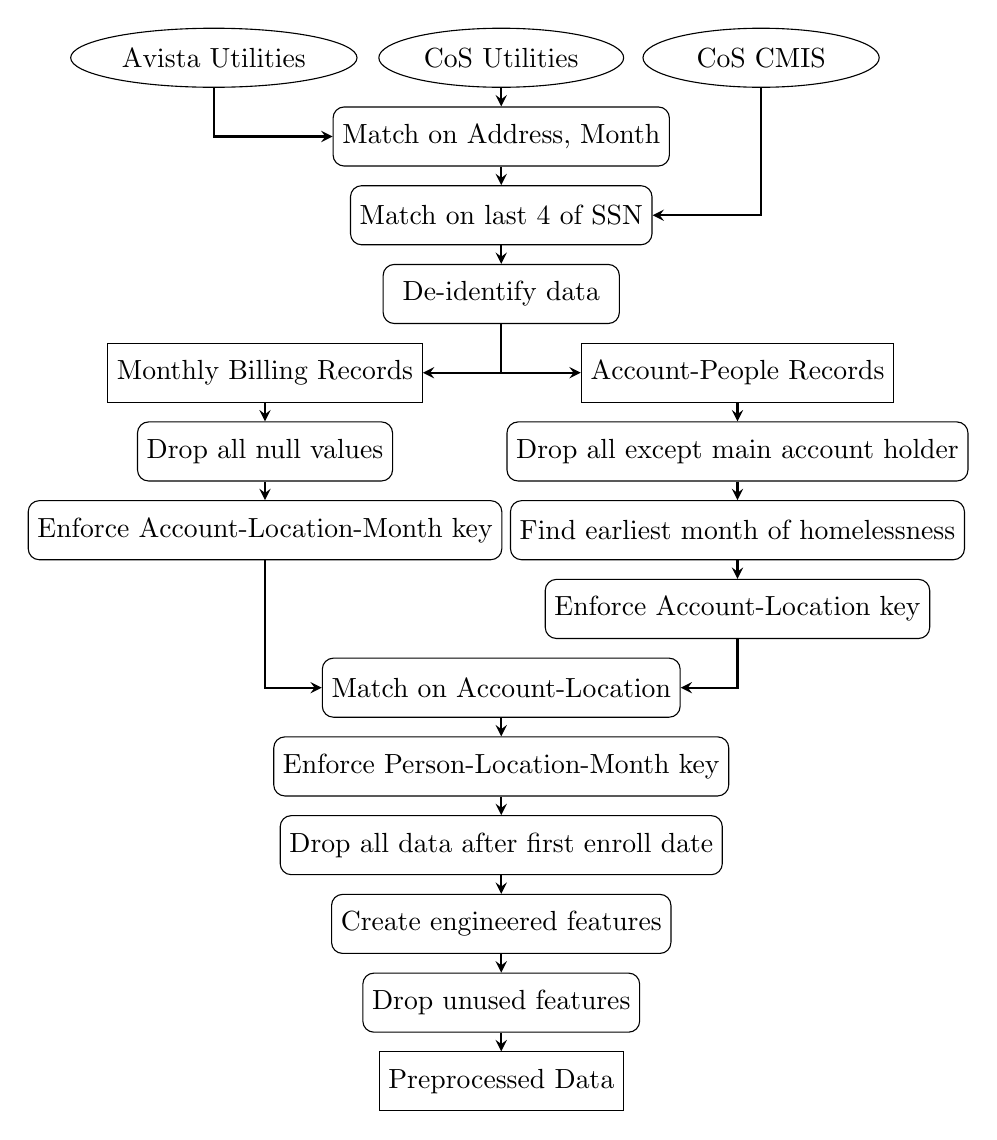
\begin{tikzpicture}[node distance=1cm]
        \node (CoSutility) [org] {CoS Utilities};
        \node (Avista) [org, left of=CoSutility, xshift=-2.65cm] {Avista Utilities};
        \node (CoScmis) [org, right of=CoSutility, xshift=2.3cm] {CoS CMIS};

        \node (Matching1) [process, below of=CoSutility] {Match on Address, Month};
        \node (Matching2) [process, below of=Matching1] {Match on last 4 of SSN};
        \node (DeID) [process, below of=Matching2] {De-identify data};

        \node (Billing) [io, below of=DeID, xshift=-3cm] {Monthly Billing Records};
        \node (Accounts) [io, below of=DeID, xshift=3cm] {Account-People Records};

        \node (bill1) [process, below of=Billing] {Drop all null values};
        \node (bill2) [process, below of=bill1] {Enforce Account-Location-Month key};
        \node (acct1) [process, below of=Accounts] {Drop all except main account holder};
        \node (acct2) [process, below of=acct1] {Find earliest month of homelessness};
        \node (acct3) [process, below of=acct2] {Enforce Account-Location key};
        
        \node (match3) [process, below of=acct3, xshift=-3cm] {Match on Account-Location};
        \node (drop1) [process, below of=match3] {Enforce Person-Location-Month key};
        \node (drop2) [process, below of=drop1] {Drop all data after first enroll date};
        \node (create) [process, below of=drop2] {Create engineered features};
        \node (drop3) [process, below of=create] {Drop unused features};

        \node (result) [io, below of=drop3] {Preprocessed Data};


        \draw [arrow] (Avista) |- (Matching1);
        \draw [arrow] (CoSutility) -- (Matching1);
        \draw [arrow] (Matching1) -- (Matching2);
        \draw [arrow] (CoScmis) |- (Matching2);
        \draw [arrow] (Matching2) -- (DeID);

        \draw [arrow] (DeID) |- (Billing);
        \draw [arrow] (DeID) |- (Accounts);
        \draw [arrow] (Billing) -- (bill1);
        \draw [arrow] (bill1) -- (bill2);
        \draw [arrow] (bill2) |- (match3);
        \draw [arrow] (Accounts) -- (acct1);
        \draw [arrow] (acct1) -- (acct2);
        \draw [arrow] (acct2) -- (acct3);
        \draw [arrow] (acct3) |- (match3);

        \draw [arrow] (match3) -- (drop1);
        \draw [arrow] (drop1) -- (drop2);
        \draw [arrow] (drop2) -- (create);
        \draw [arrow] (create) -- (drop3);
        \draw [arrow] (drop3) -- (result);
\end{tikzpicture}
\end{figure}

\begin{figure}[!h]
    \centering
    \subfloat[Threshold = 0.60 (Large Net)]{
        \begin{NiceTabular}{|c|c|c|} \hline
            Prediction & Binned & Actual \\ \hline
            \rowcolor{lightgray}
            0.98 & 1 & 1 \\ \hline
            \rowcolor{lightgray}
            0.92 & 1 & 1 \\ \hline
            0.91 & 1 & 0 \\ \hline
            \rowcolor{lightgray}
            0.84 & 1 & 1 \\ \hline
            0.73 & 1 & 0 \\ \hline \hline
            0.54 & 0 & 1 \\ \hline
            \rowcolor{lightgray}
            0.53 & 0 & 0 \\ \hline
            \rowcolor{lightgray}
            0.48 & 0 & 0 \\ \hline
            \vdots & \vdots & \vdots \\ \hline
        \end{NiceTabular}
    }
    \qquad
    \subfloat[Threshold = 0.80 (Small Net)]{
        \begin{NiceTabular}{|c|c|c|} \hline
            Prediction & Binned & Actual \\ \hline
            \rowcolor{lightgray}
            0.98 & 1 & 1 \\ \hline
            \rowcolor{lightgray}
            0.92 & 1 & 1 \\ \hline
            0.91 & 1 & 0 \\ \hline \hline
            0.84 & 0 & 1 \\ \hline
            \rowcolor{lightgray}
            0.73 & 0 & 0 \\ \hline
            0.54 & 0 & 1 \\ \hline
            \rowcolor{lightgray}
            0.53 & 0 & 0 \\ \hline
            \rowcolor{lightgray}
            0.48 & 0 & 0 \\ \hline
            \vdots & \vdots & \vdots \\ \hline
        \end{NiceTabular}
    }
\end{figure}

\end{document}